% ----------------------------------------------------------
% Introdução
% ----------------------------------------------------------
\chapter[Introdução]{Introdução}

A rede de computadores do mundo se tornou de longe uma das principais evoluções da humanidade. A globalização é a prova de que todo o avanço funcionou e essa evolução foi necessária. Nesse contexto, a pesquisa sobre segurança da informação foi ampliada, principalmente devido à necessidade.

Quando se tem grandes sistemas dedicados a manter informações sensíveis, seja de pessoas físicas ou jurídicas, a segurança se vê necessária. O trabalho de assegurar que informações sejam mesmo secretas é o desafio da informática. Há sempre a possibilidade de alguém sem direitos ter acesso a alguma informação, ou mesmo que o dado a ser salvo seja alterado, perdido ou modificado, esses são os riscos de se manter os dados. 

O risco pode ser definido como a probabilidade de que uma situação física com potencial de causar danos possa ocorrer, em qualquer nível, em decorrência da exposição durante um determinado espaço de tempo a uma vulnerabilidade, que por sua vez é definida como uma fraqueza em um sistema, que pode envolver pessoas, processos ou tecnologia que pode ser explorada para se obter acesso a informações \cite{Peotta2006}. 

Se as técnicas para manter a integridade de uma informação já são difícieis no contexto atual, onde inúmeros sistemas conseguem decifrar criptografias, então apresentar formas de acesso diretamente da informação dificultaria ainda mais a manutenção da segurança. Essas formas são as vulnerabilidades de sistemas e serviços, que fazem com que os atacantes tenham muito mais poder de conseguir capturar alguma informação. 

Na existência de uma vulnerabilidade tem-se um risco que decorre do surgimento de uma ameaça que definimos como qualquer circunstância ou evento com o potencial de causar impacto sobre a confidencialidade, integridade ou disponibilidade da informação \cite{Peotta2006}.

As vulnerabilidades de sistema entram em contraste com o acelerado crescimento da informática. Elas mostram como sistemas de grandes empresas podem, facilmente, perecer sob ataques. As principais fontes de dados sobre incidentes de segurança do Brasil são o Centro de Atendimento a Incidentes de Segurança (CAIS), vinculado à Rede Nacional de Pesquisa (RNP) e o Centro de Estudos, Resposta e Tratamento de Incidentes de Segurança no Brasil (CERT.br). Dados dessas instituições mostram que os incidentes de segurança apresentam uma forte tendência de crescimento e cada vez maior impacto. A revolução digital, desenvolvimento das tecnologias e o crescimento das vendas de dispositivos com acesso à Internet são alguns dos fatores que podem explicar este crescimento \cite{Miani2013}.

A Figura \ref{fig:intro1} mostra em resumo o número de vulnerabilidades encontradas no dia 24/10/2019, na semana corrente à essa data, nos meses 10/2019 e 09/2019 e no ano de 2019. 

\begin{figure}[H]
\centering
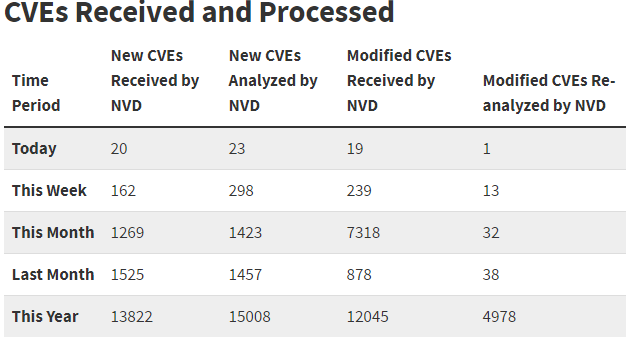
\includegraphics[width=1\textwidth]{imagens/grafico_cve.png}
\caption{Vulnerabilidades anunciadas recentemente}
\label{fig:intro1}
\end{figure}

Ainda como exemplo, a figura \ref{fig:intro2} apresenta a quantidade de vulnerabilidades já sumarizadas e interpretadas de acordo com sua complexidade o quão críticas são.

\begin{figure}[H]
\centering
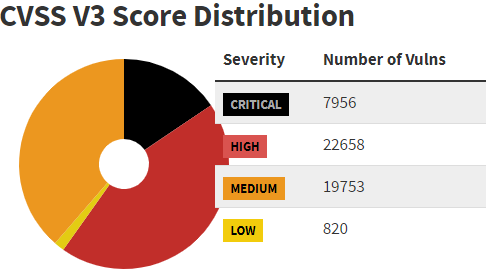
\includegraphics[width=1\textwidth]{imagens/grafico_cve_score.png}
\caption{Gráfico que contabiliza um total de vulnerabilidades já interpretadas no ano de 2019}
\label{fig:intro2}
\end{figure}

O número de vulnerabilidades que são encontradas em sistemas, nos últimos anos, cresceu de forma exponencial. Isso não significa que todas descobertas foram exploradas. A grande quantidade de demanda para uma baixa quantidade de produção de reparos faz com que apenas vulnerabilidades julgadas como críticas sejam exploradas, uma vez que as restantes são deixadas de lado.

Vulnerabilidades em softwares têm sido amplamente utilizadas por atacantes, para roubo de informações confidenciais e invasões de redes corporativas. Prover a segurança de um software, porém, não é um objetivo fácil de ser alcançado, dada a complexidade dos sistemas nos dias de hoje \cite{Uto2009}.

Os atacantes que encontram essas vulnerabilidades, em sua essência, mostram seus poderes em redes sociais apresentando seus ataques e compartilhando alguns dados recolhidos. Muitas vezes disponibilizam até instruções de como fazer o ataque. Alguns pedem para outros usuários instalarem aplicativos em suas máquinas para ajudar nos ataques, assim suas máquinas atuam como bootnets.

No contexto da segurança de computadores, vulnerabilidades são falhas ou fraquezas de softwares que permitem a agentes maliciosos subverterem o uso originalmente desejado de algum sistema computacional e violarem políticas de segurança. 

Um software seguro é aquele que satisfaz os requisitos implícitos e explícitos de segurança em condições normais de operação e em situações decorrentes de atividade maliciosa de usuários \cite{Uto2009}. Cada fase de um ciclo de desenvolvimento de software seguro, portanto, tem sua parcela de contribuição para a qualidade do resultado final e não pode ser omitida durante o processo. Na etapa de especificação, requisitos explícitos de segurança devem ser enumerados e requisitos funcionais devem ser avaliados, para verificar se não introduzem uma vulnerabilidade no sistema \cite{Uto2009}.

Sistemas inteiros podem ser tomados por crakers, que conseguem ter informações sigilosas sobre os usuários de um serviço, ou mesmo da empresa que mantém tal sistema. Além disso, crakers muitas vezes estorquem empresas a pagarem elevadas quantias para terem seus sistemas e dados privados de volta. 

A discussão sobre as vulnerabilidades em redes sociais mostram como o assunto é tomado pelo público. Assim, pessoas passam a entender mais sobre sistemas e seus bugs, começam a identificar quais são as formas de se identificar vulnerabilidades e quais os passos para apresenta-las ao mundo para que sejam exploradas de maneira legal.

O número de pessoas que discutem temas como vulnerabilidades e bugs em sistemas têm crescido assim como o número de vulnerabilidades. O foco é conseguir reduzir o número de falhas em sistemas. A discussão do tema leva as pessoas a entenderem mais sobre o assunto, assim mais pessoas contribuem em encontrar falhas em serviços e sistemas.

A exploração de uma vulnerabilidade descoberta em um sistema ou serviço faz surgir uma ameaça. Essa, é tratada já como a concretização de um ataque. Uma ameaça consiste em uma possível ação que, se concretizada, poderá produzir efeitos indesejados ao sistema, comprometendo a confidencialidade, a integridade, a disponibilidade e/ou a autenticidade. Já o ataque é a concretização de uma ameaça, através da exploração de alguma vulnerabilidade do sistema, executado por algum intruso de forma maliciosa ou não \cite{Mello2006}.

Apesar de todo o investimento realizado contra as ameaças à segurança da informação, a quantidade de ataques a empresas e seus aplicativos vem aumentando mais rapidamente do que a nossa capacidade em poder enfrentá-los \cite{ALVESBATISTA2007}.

O objetivo desse trabalho é identificar as vulnerabilidades que são discutidas na rede social do twitter, tais como seus aspectos e a possibilidade de ser exploradas. O foco é analisar o volume de dados de discussão sobre esse tópico na rede social, a fim de entender se há um aumento na atenção desse assunto. Como nos últimos anos houve um notável aumento no volume de vulnerabilidades- espera-se que o aumeto de pessoas interessadas também tenha evoluído. Será criado um sistema que fará uma busca na API GetOldTweets \cite{Pythoncommunity} através de filtros pré selecionados afim de conseguir uma base de dados para verificação dos tweets a partir de tal busca. Assim, com o sistema criado, será feito uma análise dos dados para levantar, quantativa e qualitativamente os dados de segurança discutidos no Twitter tendo em vista as vulnerabilidades já exploradas.

Com a criação desse sistema que consiga fazer uma busca no twiter através de alguns parâmetros, como palavras chaves, filtro de data etc, o objetivo é capturar o resultado em um arquivo e nele fazer uma mineração de dados para identificar palavras recorrentes. Com uma busca de índice invertido, ainda, identificar quais são as palavras recorrentes e combina-las com as vulnerailidaes já conhecidas pelo CVE.

Afim de listar as vulnerabilidades discutidas e o volume dessas informações, será possível com o sistema, através de mineração de dados, identificar quais são as vulnerabilidades mais discutidas, quais os usuários que normalmente fazem tais publicações e o quão retwitadas elas são na rede social.

% ------------------%
% --- Objetivos --- %
%\section{Objetivos}


% -------------------%
% --- Resultados --- %
%\section{Resultados esperados}

%\section{Organização do Trabalho}
